\section{Hands-on experience}


% What did you choose to experiment with and why?

A more classic machine learning approach has been applied to partially reproduce the study. An extremely randomised decision tree (or Extra-Tree) \cite{geurts_extremely_2006} model has been fit to perform fully automatic vascular segmentation on one of the datasets used in the study, the DRIVE dataset \cite{staal_ridge-based_2004}. This approach has been chosen for its simplicity to implement using scikit-learn \cite{pedregosa_scikit-learn:_2011}.


% Explain your setup

The DRIVE dataset consists on 20 training samples and 20 test samples. Each sample is composed on a retinal fundus image, an asocciated mask corresponding to the circular field of view and manual segmentations by human experts (one for the training samples and two for the test samples).

The code used to run the experiments and generate the figures is available online\footnote{\href{https://github.com/fepegar/cast-coursework}{https://github.com/fepegar/cast-coursework}}. The 12 pixel-wise features used for classification are the 3 RGB channels, the 3 HSV channels, the 3 L*a*b* channels, a Frangi vesselness filter \cite{frangi_multiscale_1998}, a Sobel filter and a Laplacian filter. The model has been trained using different weights for the foreground (vessels) and background (rest) classes, since most of the masked pixels of each label image are part of the background (87\% $\pm$ 2\%). The weights are automatically calculated by the classifier. Predictions are saved the probability of a pixel belonging to the foreground class.


% Report the results you obtained. Negative results are also interesting

Figure \ref{fig:collage} shows the segmentation results for the samples with highest, median and lowest Dice scores between the probability maps thresholded at 0.5 and the first manual segmentation. Most of the false negatives are smaller vessels, and most of the false positives are noisy predictions of isolated images. In DRIU, most of the false negatives are small vessels that were segmented by only one of the annotators, while most of the false positives are borders around the thinner vessels.

\begin{figure}
  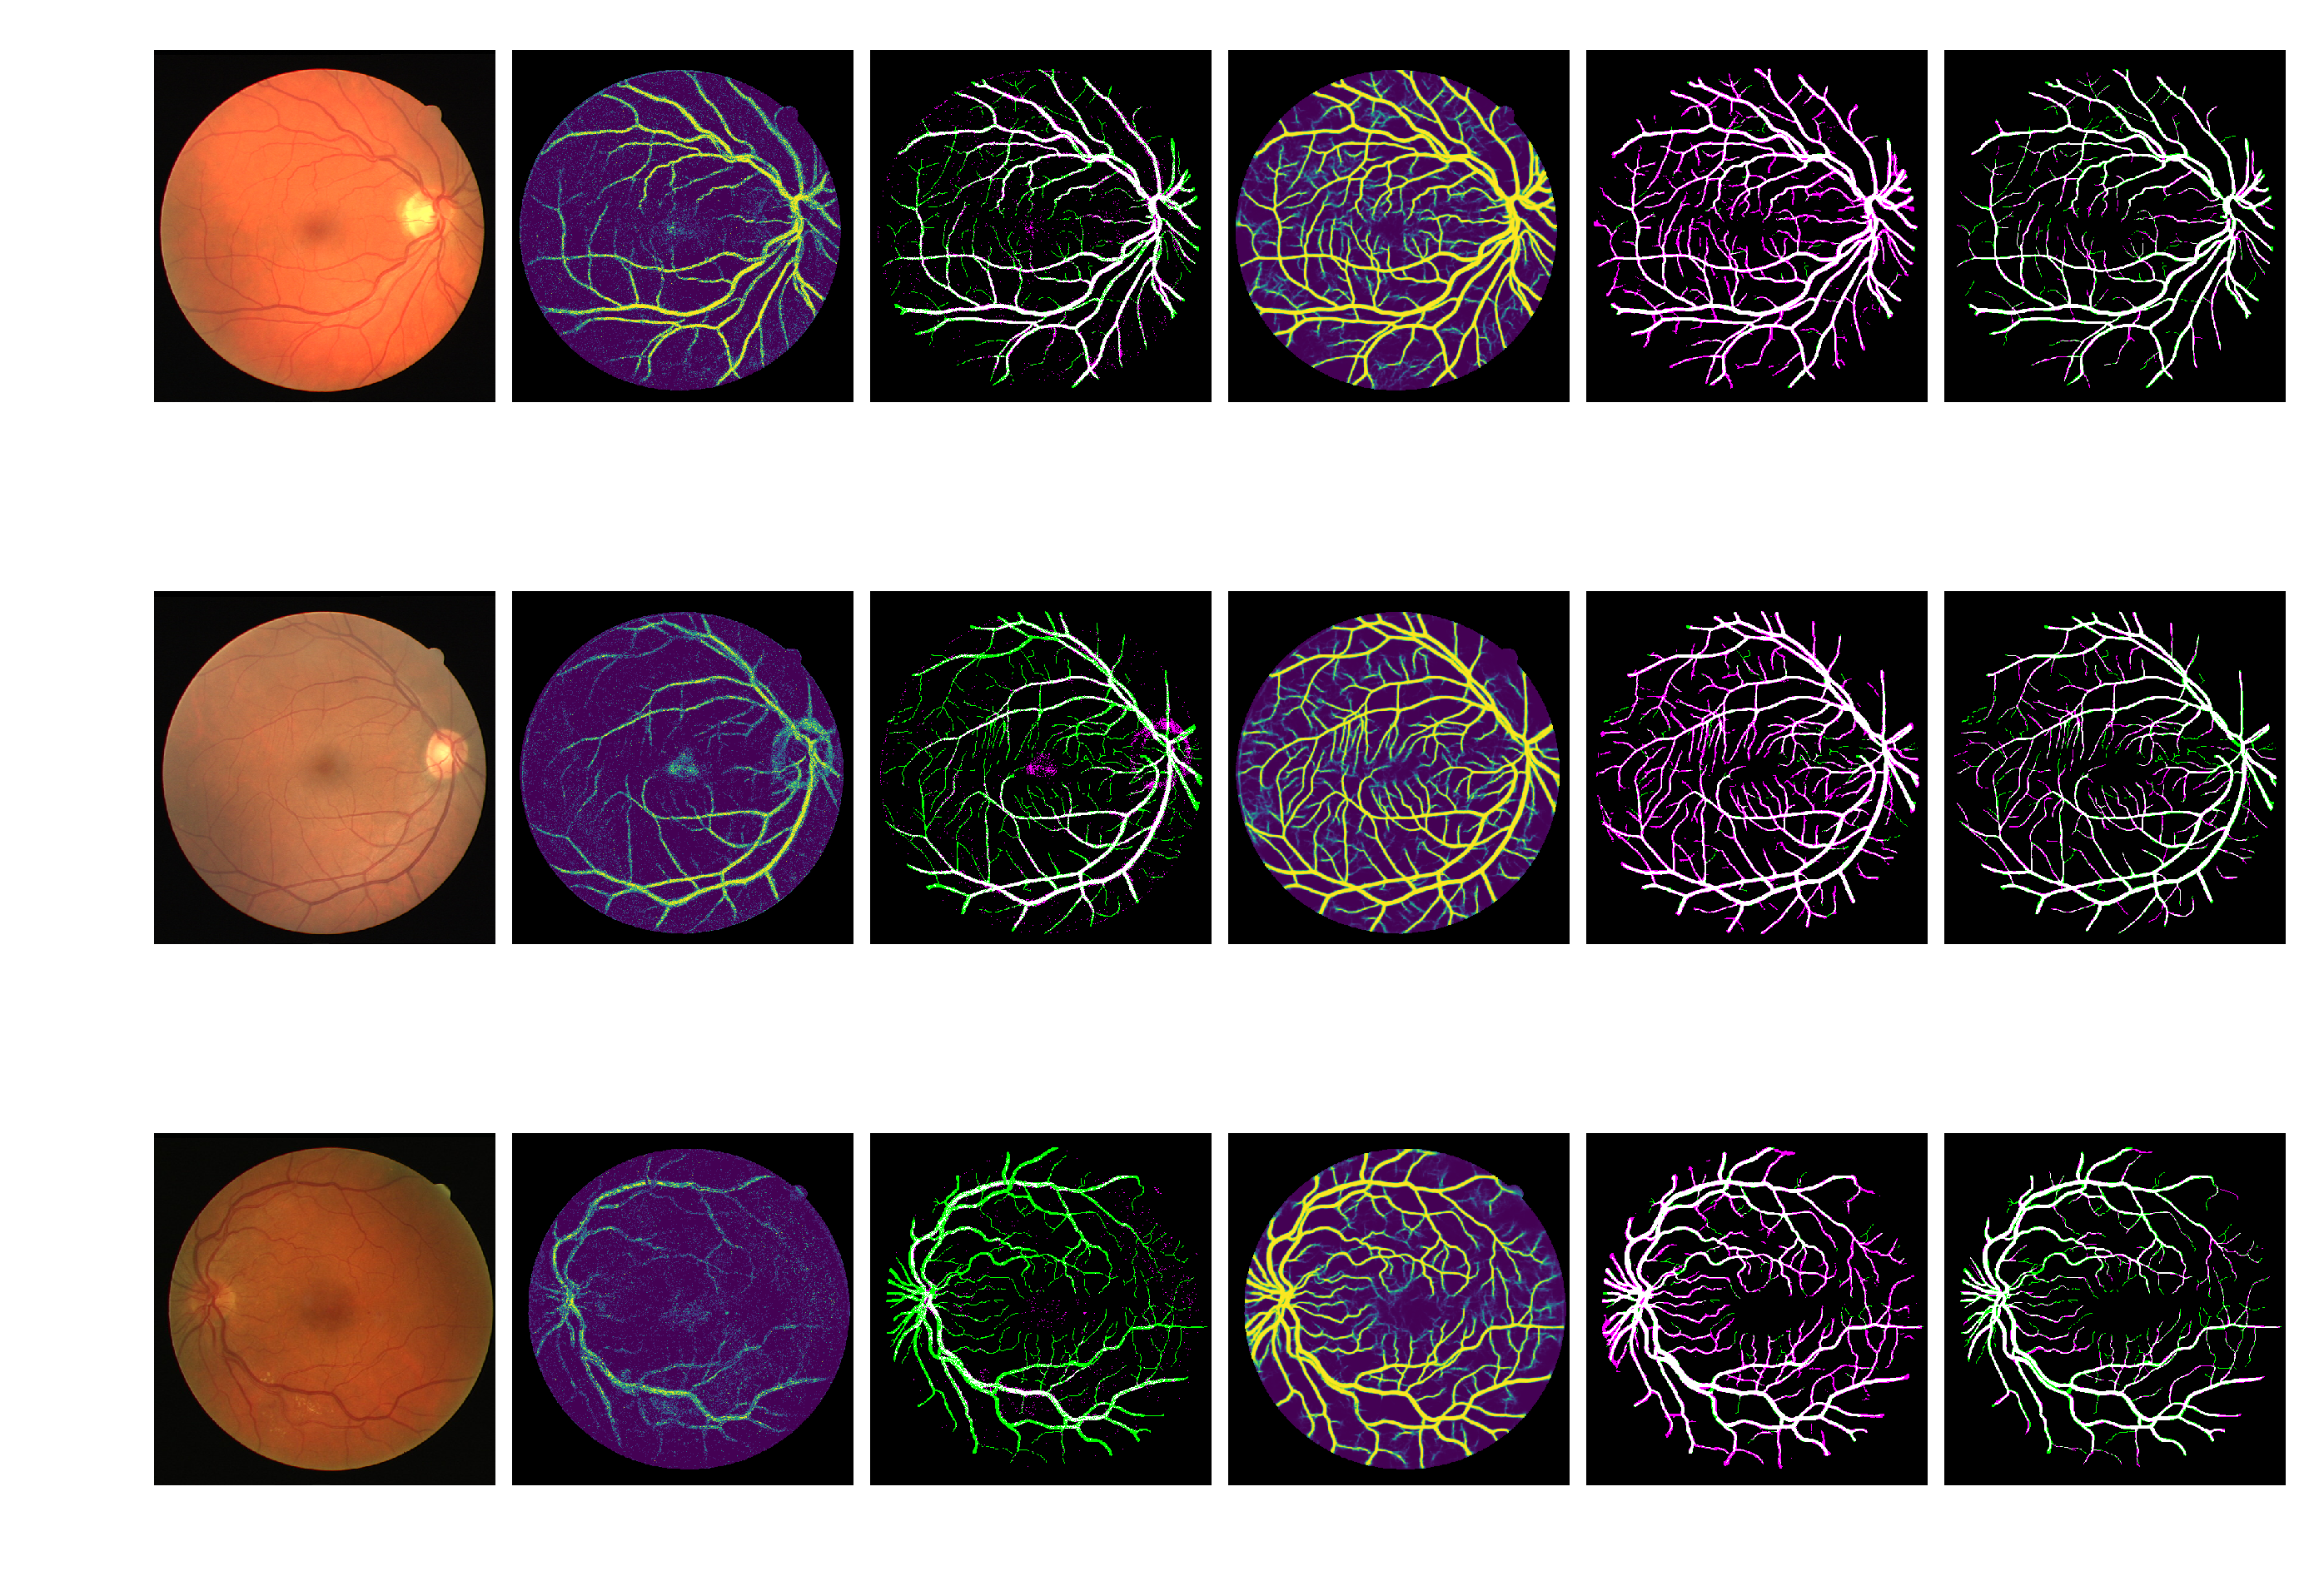
\includegraphics[width=\textwidth]{figures/collage}
  \caption{Results with highest (top), median (middle) and lowest (bottom) Dice scores using a 0.5 threshold. From left to right: acquired image of the retinal fundus; vessel probabilities using Extra-Trees; comparison of Extra-Trees thresholded probabilities to manual segmentation; vessel probabilities using DRIU; comparison of DRIU thresholded probabilities to manual segmentation; comparison of manual segmentation from first and second annotators. When comparing binary images: first annotator is used as ground truth; white pixels represent true positives; black pixels represent true negatives; magenta pixels represent false positives; and green pixels represent false negatives. The probability maps have been masked to show only the acquired field of view and higher lightness represents higher foreground probability.}
  \label{fig:collage}
\end{figure}

Figure~\ref{fig:dice} shows a comarison of all the Dice scores for both methods. DRIU presents higher scores for all cases. Figure~\ref{fig:pr} shows the region precision-recall curve for this method. The area under the curve is much smaller than the obtained by DRIU.

\begin{figure}
  \centering
  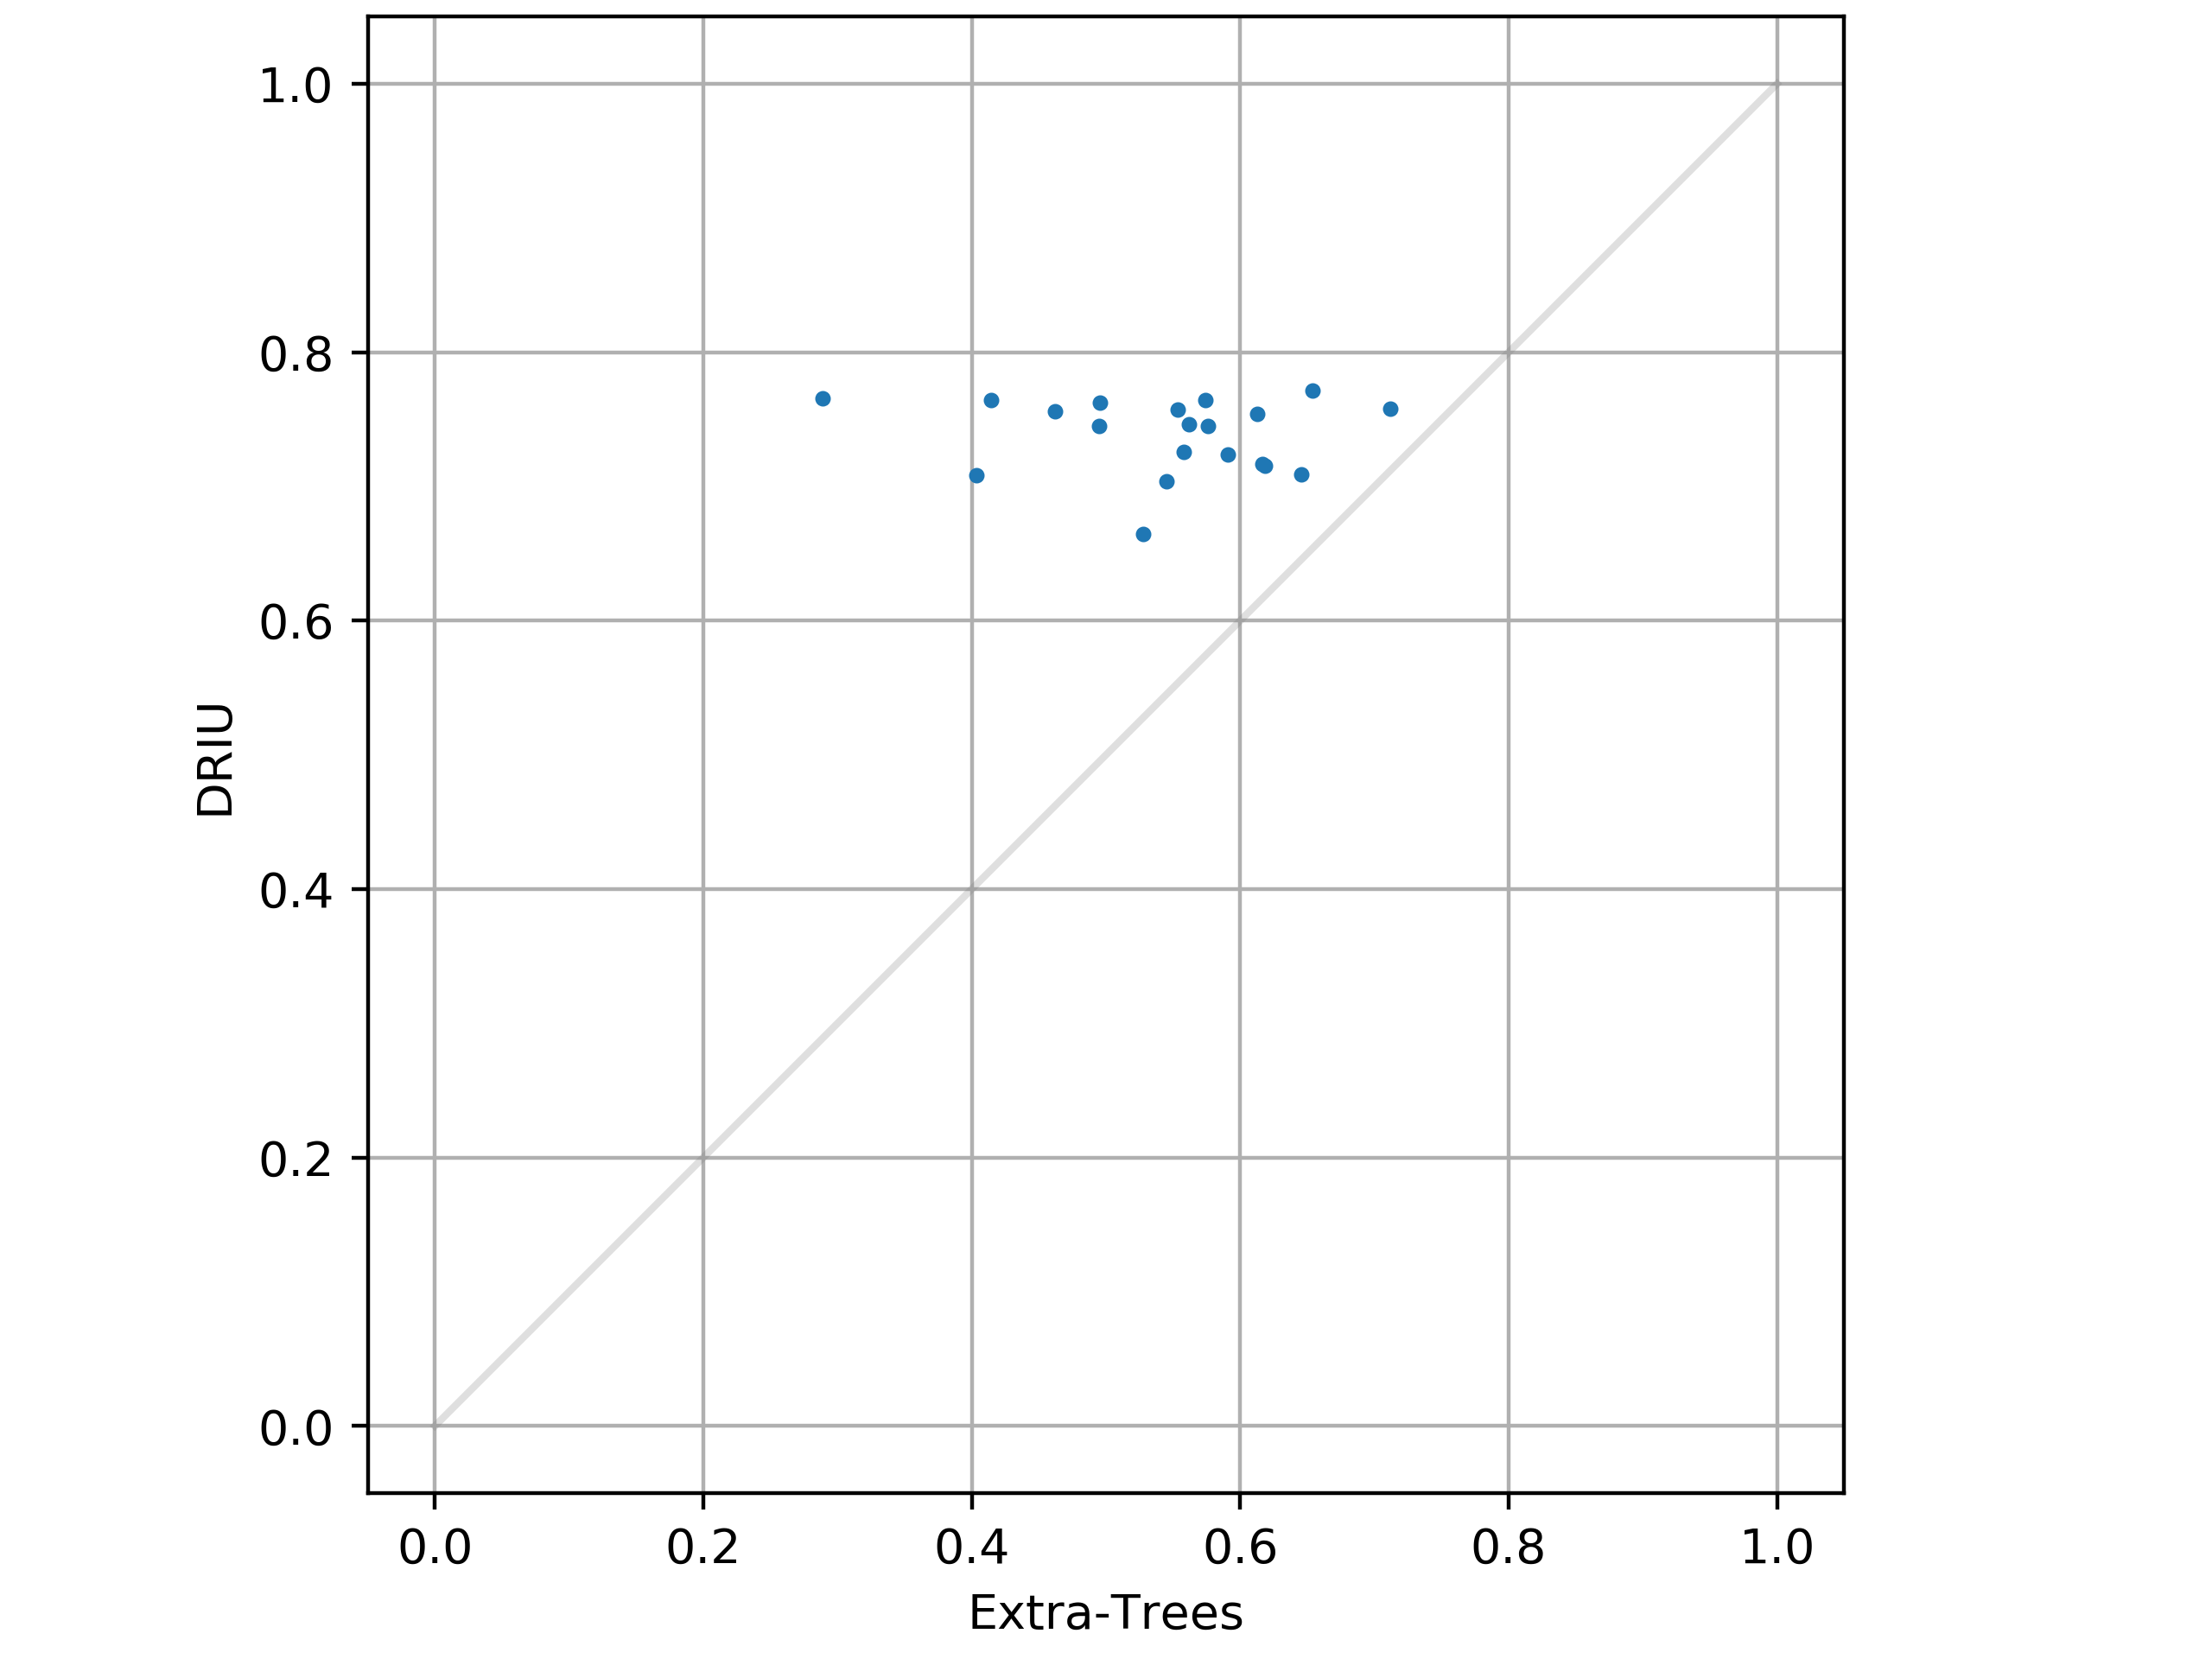
\includegraphics[width=0.6\textwidth]{figures/dices}
  \caption{Dice scores of both methods between probabilities thresholded at 0.5 and the ground truth (first annotator).}
  \label{fig:dice}
\end{figure}

\begin{figure}
  \centering
  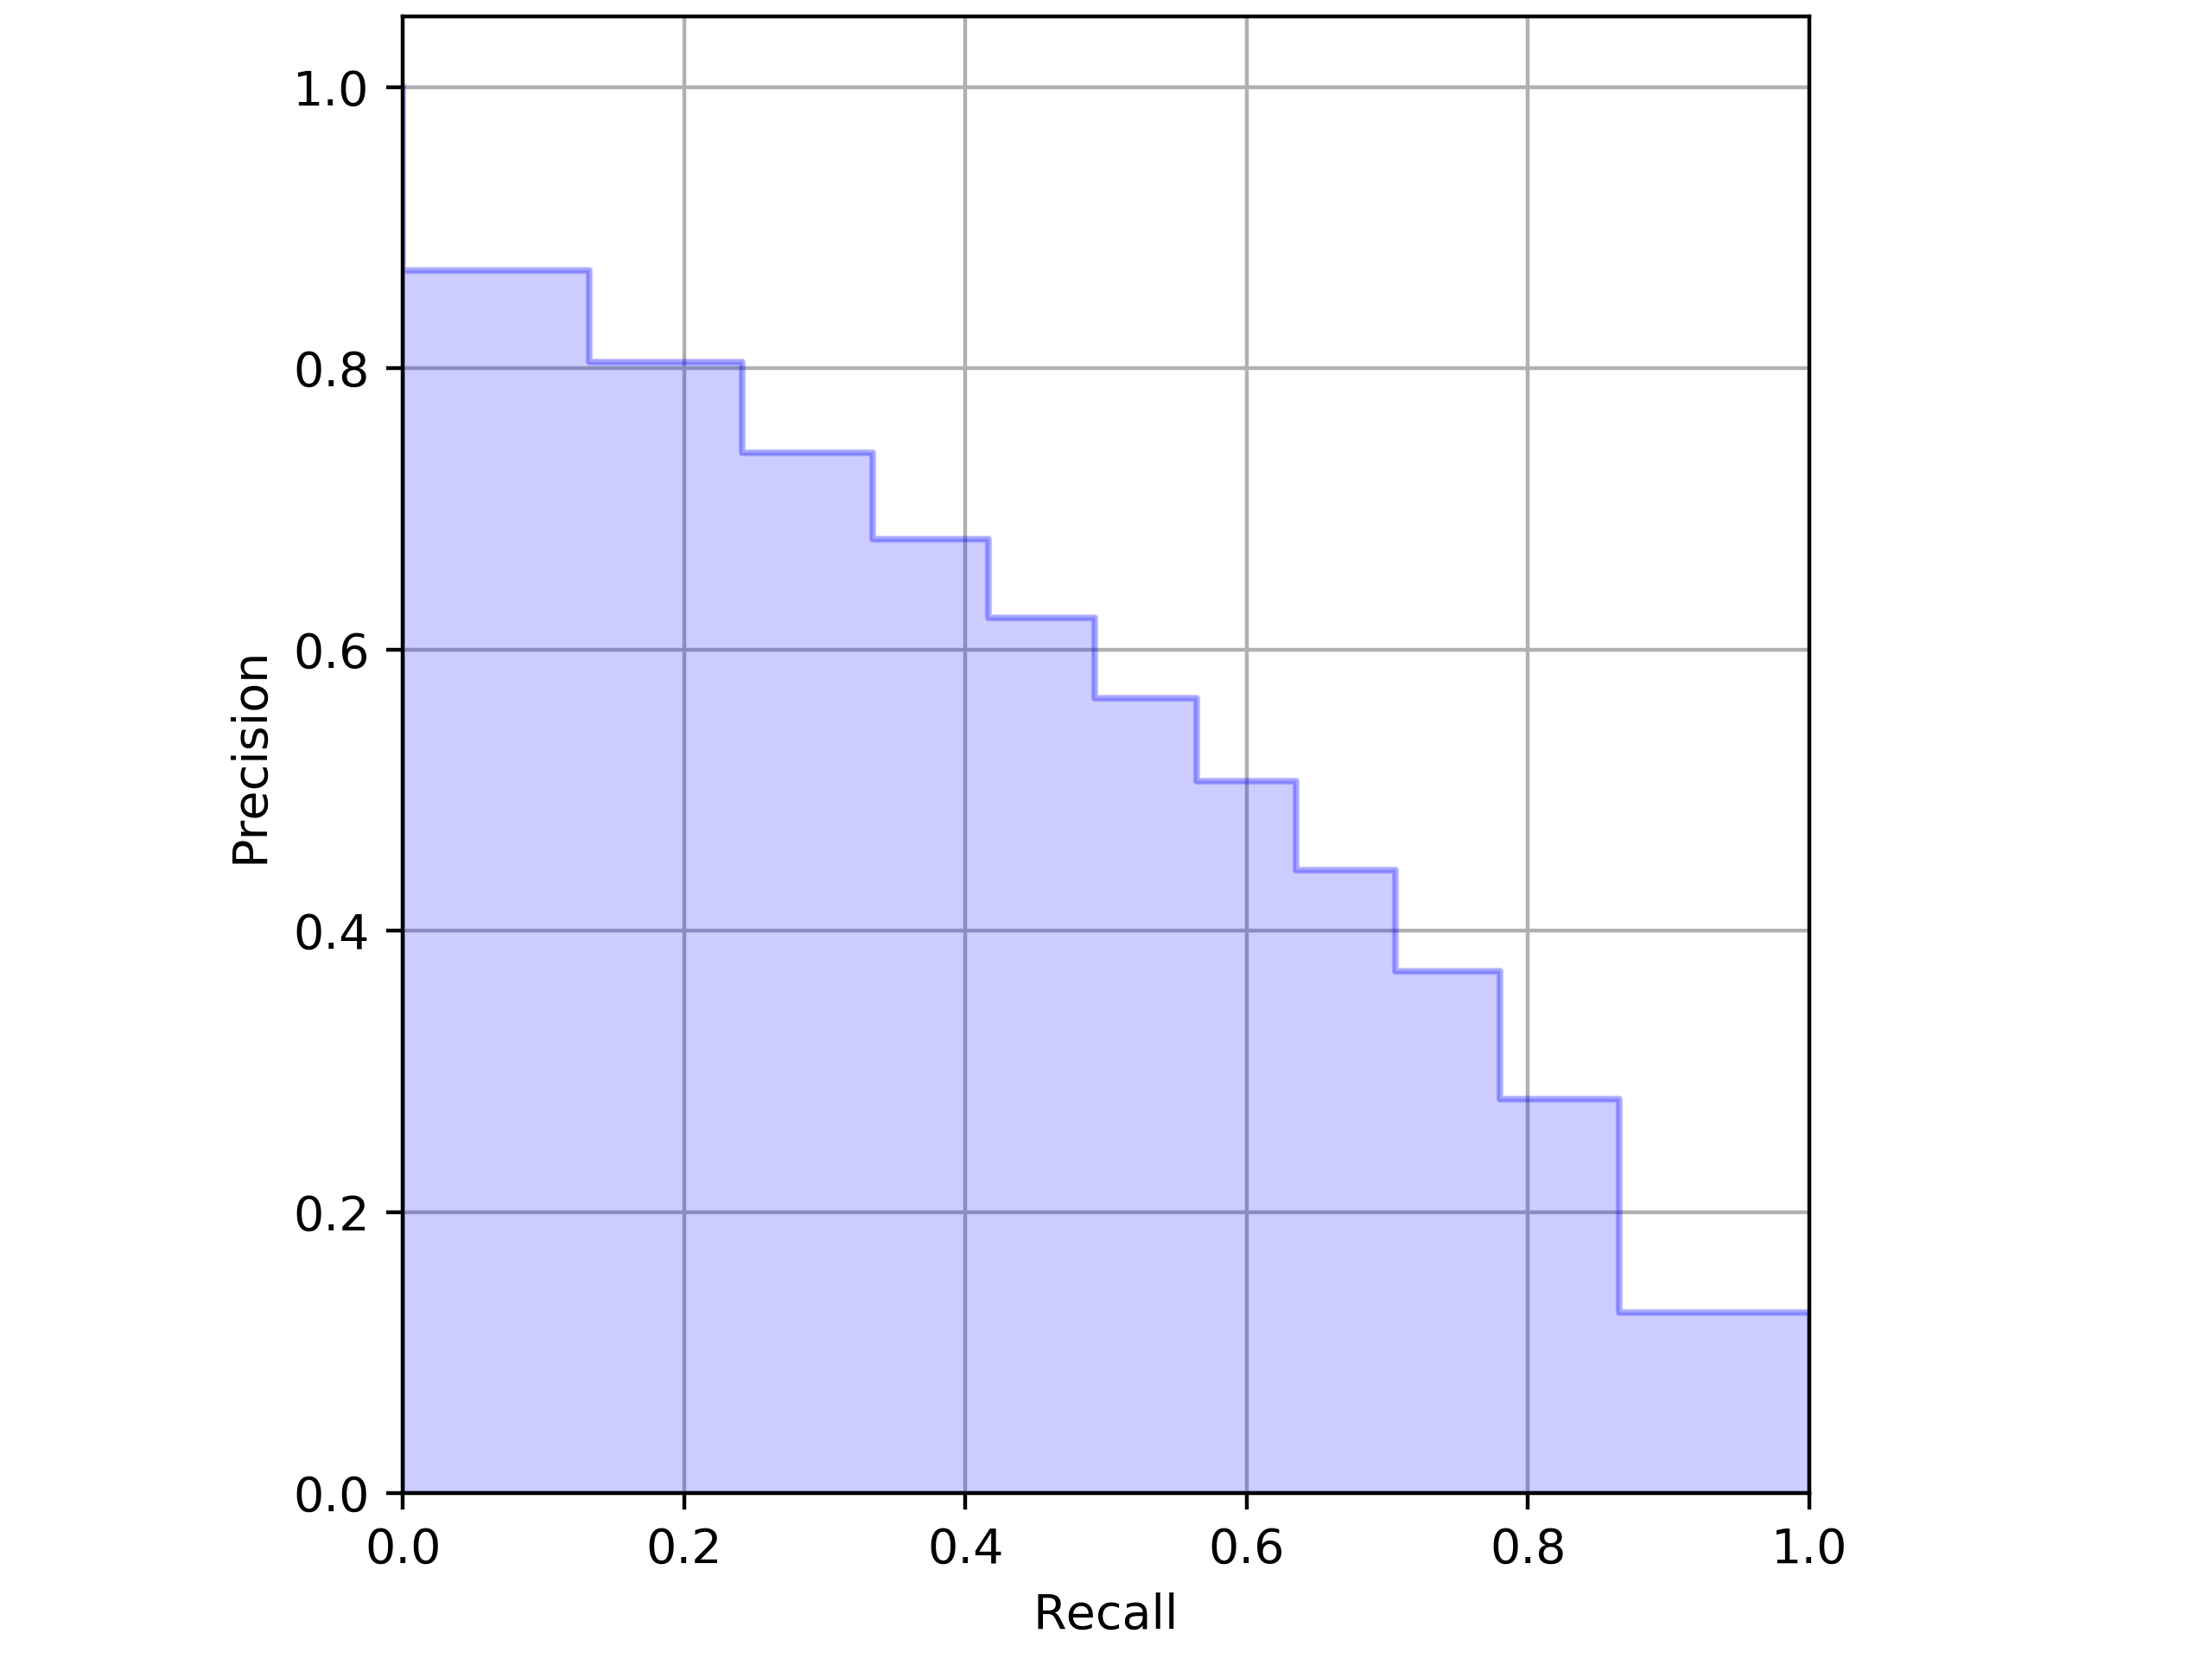
\includegraphics[width=0.8\textwidth]{figures/precision-recall}
  \caption{Region precision-recall curve between the predicted probabilities and the ground truth (first annotator).}
  \label{fig:pr}
\end{figure}

Figure~\ref{fig:importance} shows the importance of each pixel feature for the classification. As expected, the Frangi filter is the most relevant feature used by the algorithm, followed by the Sobel and Laplacian filters. The graph shows that pixels in vessels seem to be much better classified according to their spatial features, and not their colour or lightness.

\begin{figure}
  \centering
  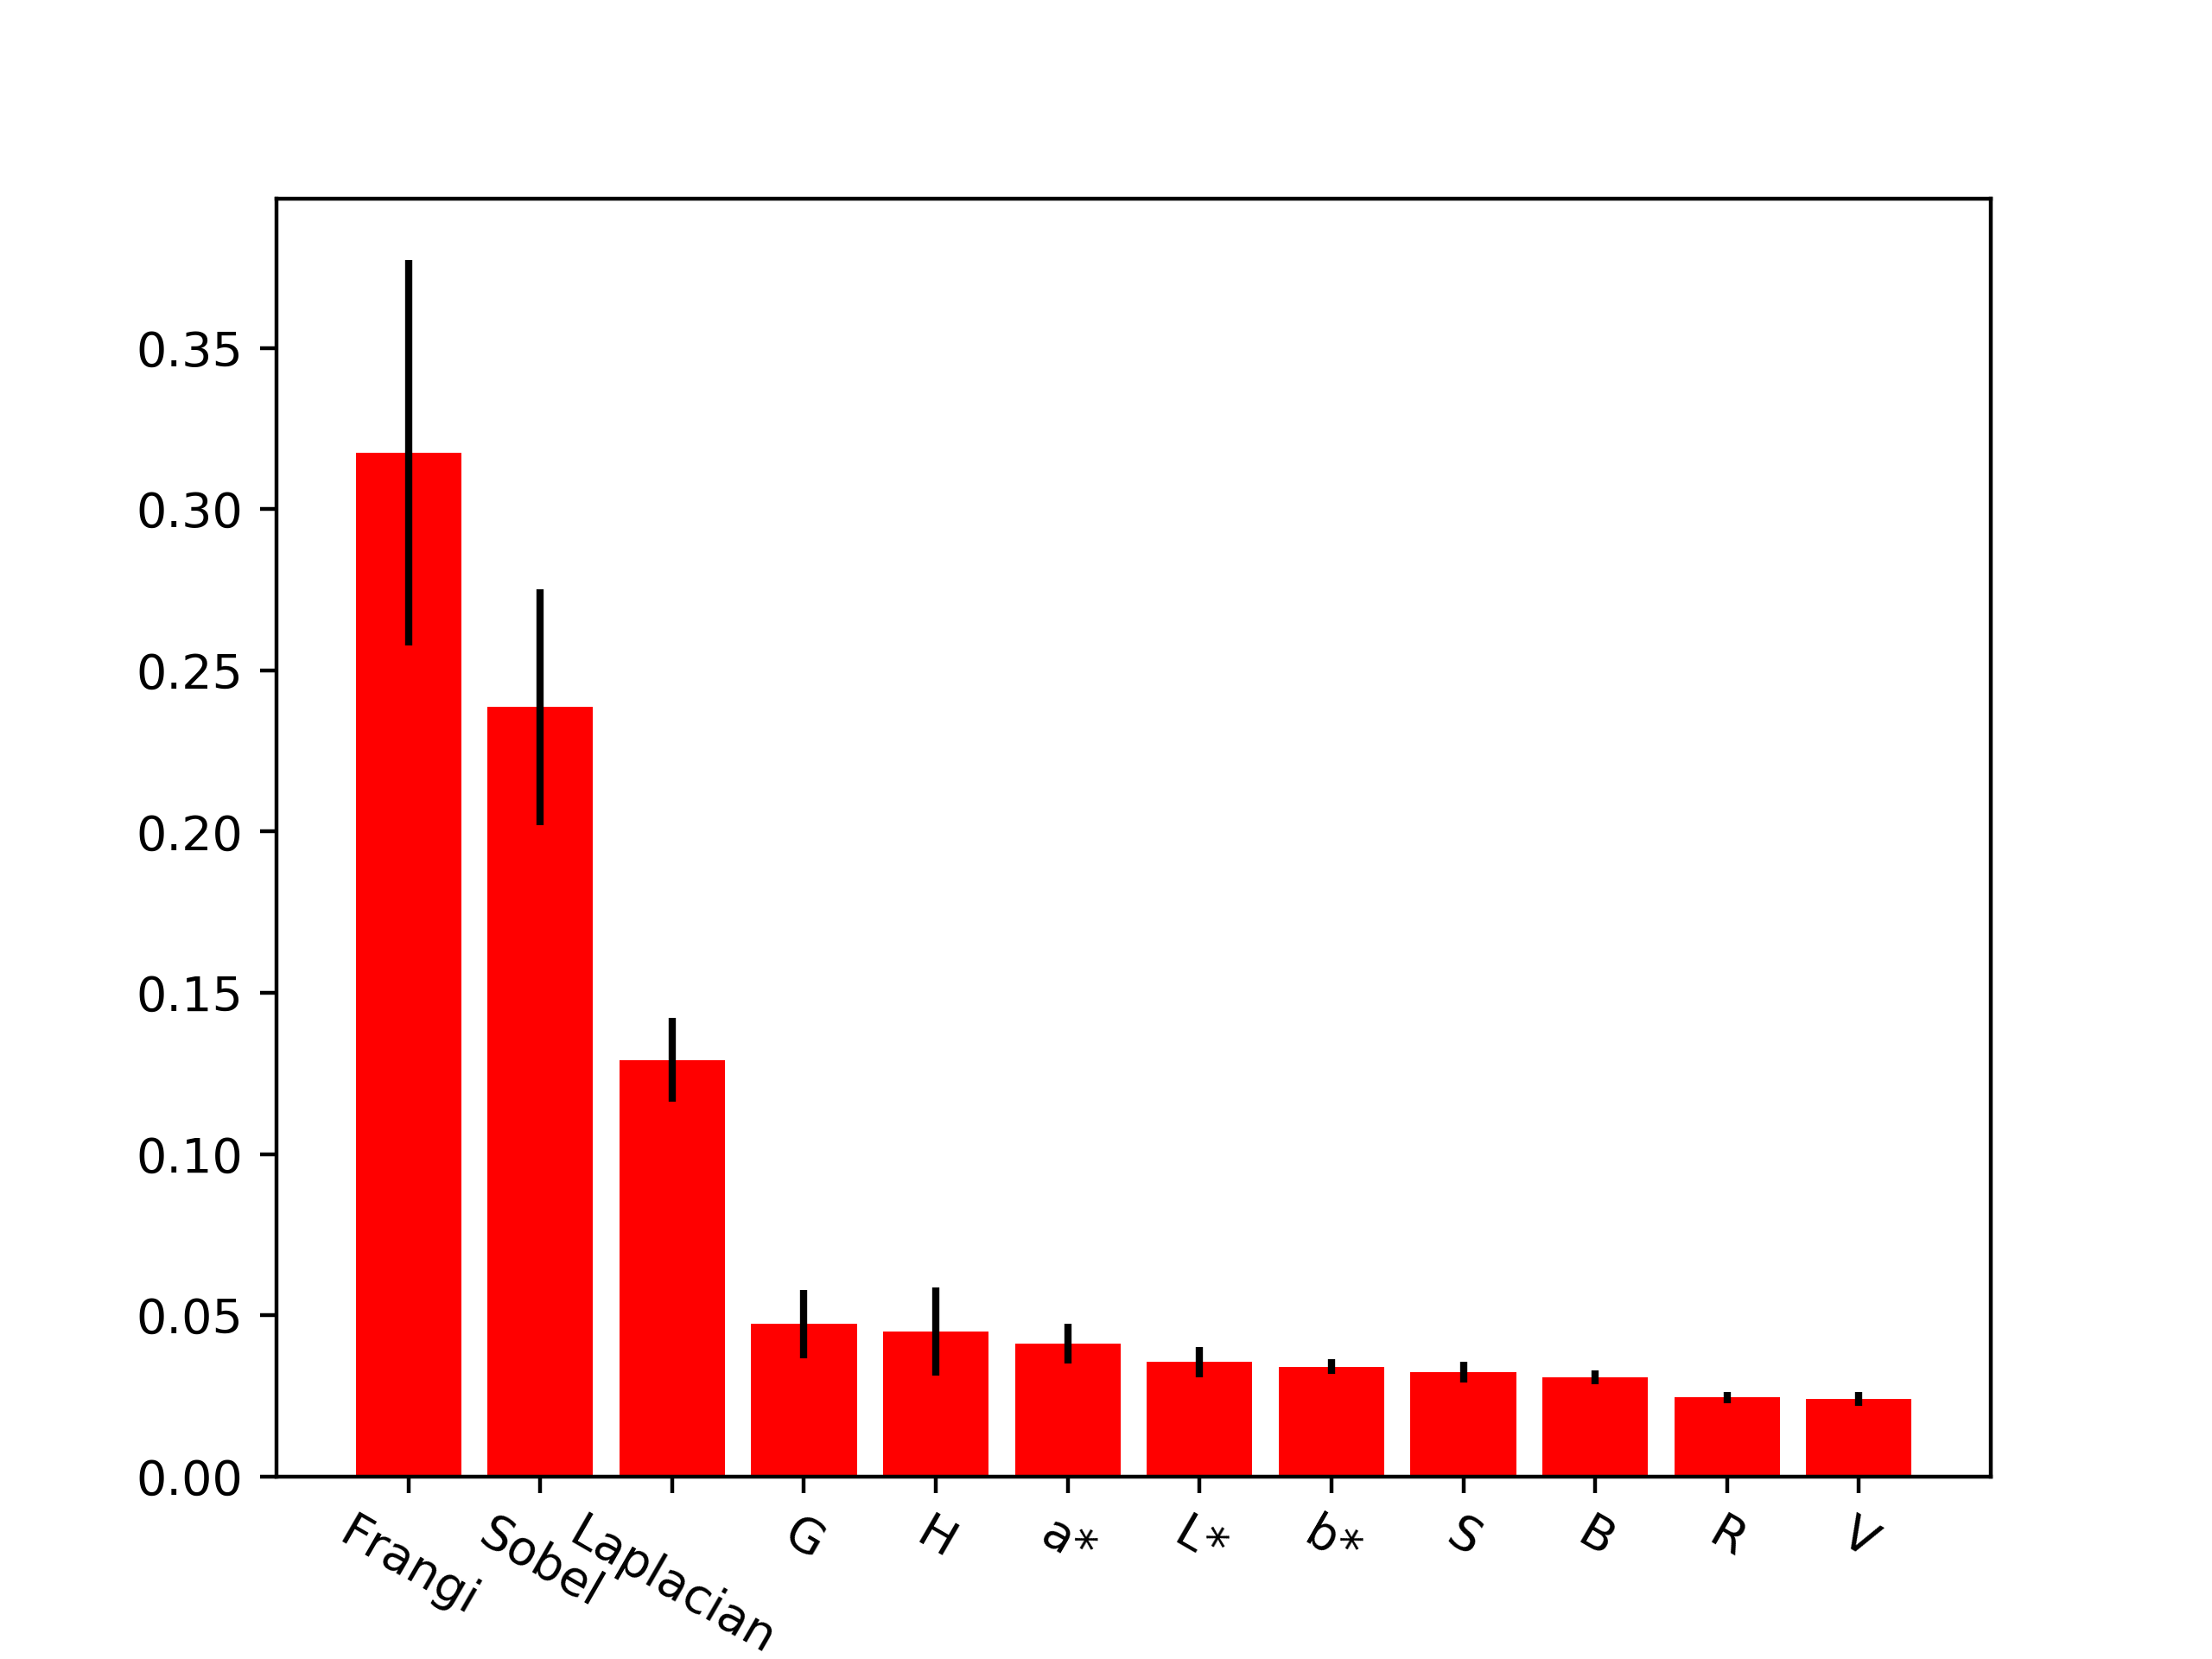
\includegraphics[width=0.8\textwidth]{figures/importances}
  \caption{Features importance for the forest, along with their inter-trees variability (standard deviation of the importance for each Extra-Trees estimator). R: red; G: green; B: blue; L: lightness; a: green-red colour component; b: blue-yellow colour component; H: hue; S: saturation; V: value.}
  \label{fig:importance}
\end{figure}
